
%{{第六十一回}}{第六十一回}}

\chapter{投鼠忌器宝玉情赃\\判冤决狱平儿情权}

{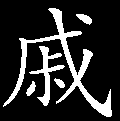
\includegraphics[width=3mm]{../Images/00005}数回用蝉脱体,络绎写来,读者几不辨何自起、何自结,浩浩无涯。须看他争端起自环哥,却起自彩云。争端结自宝玉,却亦结自彩云。首尾收束精严,六花长蛇阵也。识者着眼。}

那柳家的笑道:``好猴儿崽子!你亲婶子找野老儿去了,你岂不多得一个叔叔,有什么疑的!别讨我把你头上的杩子盖似的几根屄毛撏下来!还不开门让我进去呢。''这小厮且不开门,且拉着笑说:``好婶子,你这一进去,好歹偷些杏子出来赏我吃。我这里老等。你若忘了时,日后半夜三更打酒买油的,我不给你老人家开门,也不答应你,随你干叫去。''柳氏啐道:``发了昏的,今年不比往年,把这些东西都分给了众奶奶了。一个个的不像抓破了脸的,人打树底下一过,两眼就像那黧鸡似的,还动他的果子!昨儿我从李子树下一走,偏有一个蜜蜂儿往脸上一过,我一招手儿,偏你那好舅母就看见了。他离的远看不真,只当我摘李子呢,就屄声浪嗓喊起来,说又是`还没供佛呢',又是`老太太、太太不在家还没进鲜呢,等进了上头,嫂子们都有分的',倒像谁害了馋痨等李子出汗呢。叫我也没好话说,抢白了他一顿。可是你舅母姨娘两三个亲戚都管着,怎不和他们要去,倒和我来要。这可是`仓老鼠和老鸹去借粮------守着的没有,飞着的有'。''小厮笑道:``哎哟哟,没有罢了,说上这些闲话!我看你老以后就用不着我了?就便是姐姐有了好地方,将来更呼唤着的日子多,只要我们多答应他些就有了。''柳氏听了,笑道:``你这个小猴精,又捣鬼吊白的,你姐姐有什么好地方了?''那小厮笑道:``别哄我了,早已知道了。单是你们有内牵,难道我们就没有内牵不成?我虽在这里听哈,里头却也有两个姊妹成个体统的,什么事瞒了我们!''

正说着,只听门内又有老婆子向外叫:``小猴儿们,快传你柳婶子去罢,再不来可就误了。''柳家的听了,不顾和小厮说话,忙推门进去,笑说:``不必忙,我来了。''一面来至厨房------虽有几个同伴的人,他们都不敢自专,单等他来调停分派------一面问众人:``五丫头那去了?''众人都说:``才往茶房里找他们姊妹去了。''

柳家的听了,便将茯苓霜搁起,且按着房头分派菜馔。忽见迎春房里小丫头莲花儿走来{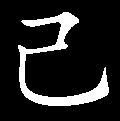
\includegraphics[width=3mm]{../Images/00003}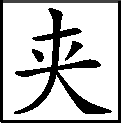
\includegraphics[width=3mm]{../Images/00012}\footnotesize \kaishu 总是写春景将残。}说:``司棋姐姐说了,要碗鸡蛋,炖的嫩嫩的。''柳家的道:``就是这样尊贵。不知怎的,今年这鸡蛋短的很,十个钱一个还找不出来。昨儿上头给亲戚家送粥米去,四五个买办出去,好容易才凑了二千个来。我那里找去?你说给他,改日吃罢。''莲花儿道:``前儿要吃豆腐,你弄了些馊的,叫他说了我一顿。今儿要鸡蛋又没有了。什么好东西,我就不信连鸡蛋都没有了,别叫我翻出来。''一面说,一面真个走来,揭起菜箱一看,只见里面果有十来个鸡蛋,说道:``这不是?你就这么利害!吃的是主子的,我们的分例,你为什么心疼?又不是你下的蛋,怕人吃了。''柳家的忙丢了手里的活计,便上来说道:``你少满嘴里混唚!你娘才下蛋呢!通共留下这几个,预备菜上的浇头。姑娘们不要,还不肯做上去呢,预备接急的。你们吃了,倘或一声要起来,没有好的,连鸡蛋都没了。你们深宅大院,水来伸手,饭来张口,只知鸡蛋是平常物件,那里知道外头买卖的行市呢。别说这个,有一年连草根子还没了的日子还有呢。我劝他们,细米白饭,每日肥鸡大鸭子,将就些儿也罢了。吃腻了膈,天天又闹起故事来了。鸡蛋、豆腐,又是什么面筋、酱萝卜炸儿,敢自倒换口味。只是我又不是答应你们的,一处要一样,就是十来样。我倒别伺候头层主子,只预备你们二层主子了。''

莲花听了,便红了脸,喊道:``谁天天要你什么来?你说上这两车子话!叫你来,不是为便宜却为什么。前儿小燕来,说晴雯姐姐要吃芦蒿,你怎么忙的还问肉炒鸡炒?小燕说:`荤的因不好才另叫你炒个面筋的,少搁油才好。'你忙的倒说自己发昏,赶着洗手炒了,狗颠儿似的亲捧了去。今儿反倒拿我作筏子,说我给众人听。''柳家的忙道:``阿弥陀佛!这些人眼见的。别说前儿一次,就从旧年一立厨房以来,凡各房里偶然间不论姑娘姐儿们要添一样半样,谁不是先拿了钱来,另买另添。有的没的,名声好听,说我单管姑娘厨房省事,又有剩头儿,算起账来,惹人恶心:连姑娘带姐儿们四五十人,一日也只管要两只鸡,两只鸭子,十来斤肉,一吊钱的菜蔬。你们算算,够作什么的?连本项两顿饭还撑持不住,还搁的住这个点这样,那个点那样,买来的又不吃,又买别的去。既这样,不如回了太太,多添些分例,也像大厨房里预备老太太的饭,把天下所有的菜蔬用水牌写了,天天转着吃,吃到一个月现算倒好。连前儿三姑娘和宝姑娘偶然商议了要吃个油盐炒枸杞芽儿来,现打发个姐儿拿着五百钱来给我,我倒笑起来了,说:`二位姑娘就是大肚子弥勒佛,也吃不了五百钱的去。这三二十个钱的事,还预备的起。'赶着我送回钱去,到底不收,说赏我打酒吃,又说:`如今厨房在里头,保不住屋里的人不去叨登,一盐一酱,那不是钱买的。你不给又不好,给了你又没的赔。你拿着这个钱,全当还了他们素日叨登的东西窝儿。'这就是明白体下的姑娘,我们心里只替他念佛。没的赵姨奶奶听了又气不忿,又说太便宜了我,隔不了十天,也打发个小丫头子来寻这样寻那样,我倒好笑起来。你们竟成了例,不是这个,就是那个,我那里有这些赔的。''

正乱时,只见司棋又打发人来催莲花儿,说他``死在这里了,怎么就不回去?''莲花儿赌气回来,便添了一篇话,告诉了司棋。司棋听了,不免心头起火。此刻伺候迎春饭罢,带了小丫头们走来,见了许多人正吃饭,见他来的势头不好,都忙起身陪笑让坐。司棋便喝命小丫头子:``动手!凡箱柜所有的菜蔬,只管丢出来喂狗,大家赚不成。''小丫头子们巴不得一声,七手八脚抢上去,一顿乱翻乱掷的。众人一面拉劝,一面央告司棋说:``姑娘别误听了小孩子的话。柳嫂子有八个头,也不敢得罪姑娘,说鸡蛋难买是真。我们才也说他不知好歹,凭是什么东西,也少不得变法儿去。他已经悟过来了,连忙蒸上了。姑娘不信瞧那火上。''

司棋被众人一顿好言,方将气劝的渐平。小丫头们也没得摔完东西,便拉开了。司棋连说带骂,闹了一回,方被众人劝去。柳家的只好摔碗丢盘自己咕嘟了一回,蒸了一碗蛋令人送去。司棋全泼了地下了。那人回来也不敢说,恐又生事。

柳家的打发他女儿喝了一回汤,吃了半碗粥,又将茯苓霜一节说了。五儿听罢,便心下要分些赠芳官,遂用纸另包了一半,趁黄昏人稀之时,自己花遮柳隐的来找芳官。且喜无人盘问。一径到了怡红院门前,不好进去,只在一簇玫瑰花前站立,远远的望着。有一盏茶时,可巧小燕出来,忙上前叫住。小燕不知是那一个,至跟前方看真切,因问作什么。五儿笑道:``你叫出芳官来,我和他说话。''小燕悄笑道:``姐姐太性急了,横竖等十来日就来了,只管找他做什么。方才使了他往前头去了,你且等他一等。不然,有什么话告诉我,等我告诉他。恐怕你等不得,只怕关园门了。''五儿便将茯苓霜递与了小燕,又说这是茯苓霜,如何吃,如何补益,``我得了些送他的,转烦你递与他就是了。''说毕,作辞回来。

正走蓼溆一带,忽见迎头林之孝家的带着几个婆子走来,五儿藏躲不及,只得上来问好。林之孝家的问道:``我听见你病了,怎么跑到这里来?''五儿陪笑道:``因这两日好些,跟我妈进来散散闷。才因我妈使我到怡红院送家伙去。''林之孝家的说道:``这话岔了。方才我见你妈出来我才关门。既是你妈使了你去,他如何不告诉我说你在这里呢,竟出去让我关门,是何主意?可知是你扯谎。''五儿听了,没话回答,只说:``原是我妈一早教我取去的,我忘了,挨到这时我才想起来了。只怕我妈错当我先出去了,所以没和大娘说得。''

林之孝家的听他辞钝色虚,又因近日玉钏儿说那边正房内失落了东西,几个丫头对赖,没主儿,心下便起了疑。可巧小蝉、莲花儿并几个媳妇子走来,见了这事,便说道:``林奶奶倒要审审他。这两日他往这里头跑的不像,鬼鬼唧唧的,不知干些什么事。''小蝉又道:``正是。昨儿玉钏姐姐说,太太耳房里的柜子开了,少了好些零碎东西。琏二奶奶打发平姑娘和玉钏姐姐要些玫瑰露,谁知也少了一罐子。若不是寻露,还不知道呢。''莲花儿笑道:``这话我没听见,今儿我倒看见一个露瓶子。''林之孝家的正因这些事没主儿,每日凤姐使平儿催逼他,一听此言,忙问在那里。莲花儿便说:``在他们厨房里呢。''林之孝家的听了,忙命打了灯笼,带着众人来寻。五儿急的便说:``那原是宝二爷屋里的芳官给我的。''林之孝家的便说:``不管你方官圆官,现有了赃证,我只呈报了,凭你主子前辩去。''一面说,一面进入厨房,莲花儿带着,取出露瓶。恐还有偷的别物,又细细搜了一遍,又得了一包茯苓霜,一并拿了,带了五儿,来回李纨与探春。

那时李纨正因兰哥儿病了,不理事务,只命去见探春。探春已归房。人回进去,丫鬟们都在院内纳凉,探春在内盥沐,只有待书回进去。半日,出来说:``姑娘知道了,叫你们找平儿回二奶奶去。''林之孝家的只得领出来。到凤姐儿那边,先找着了平儿,平儿进去回了凤姐。凤姐方才歇下,听见此事,便吩咐:``将他娘打四十板子,撵出去,永不许进二门。把五儿打四十板子,立刻交给庄子上,或卖或配人。''平儿听了,出来依言吩咐了林之孝家的。五儿唬的哭哭啼啼,给平儿跪着,细诉芳官之事。平儿道:``这也不难,等明日问了芳官便知真假。但这茯苓霜前日人送了来,还等老太太、太太回来看了才敢打动,这不该偷了去。''五儿见问,忙又将他舅舅送的一节说了出来。平儿听了,笑道:``这样说,你竟是个平白无辜之人,拿你来顶缸。此时天晚,奶奶才进了药歇下,不便为这点子小事去絮叨。如今且将他交给上夜的人看守一夜,等明儿我回了奶奶,再做道理。''林之孝家的不敢违拗,只得带了出来交与上夜的媳妇们看守,自便去了。

这里五儿被人软禁起来,一步不敢多走。又兼众媳妇也有劝他说,不该做这没行止之事;也有抱怨说,正经更还坐不上来,又弄个贼来给我们看,倘或眼不见寻了死,逃走了,都是我们不是。于是又有素日一干与柳家不睦的人,见了这般,十分趁愿,都来奚落嘲戏他。这五儿心内又气又委屈,竟无处可诉;且本来怯弱有病,这一夜思茶无茶,思水无水,思睡无衾枕,呜呜咽咽直哭了一夜。

谁知和他母女不和的那些人,巴不得一时撵出他们去,惟恐次日有变,大家先起了个清早,都悄悄的来买转平儿,一面送些东西,一面又奉承他办事简断,一面又讲述他母亲素日许多不好。平儿一一的都应着,打发他们去了,却悄悄的来访袭人,问他可果真芳官给他露了。袭人便说:``露却是给芳官,芳官转给何人我却不知。''袭人于是又问芳官,芳官听了,唬天跳地,忙应是自己送他的。芳官便又告诉了宝玉,宝玉也慌了,说:``露虽有了,若勾起茯苓霜来,他自然也实供。若听见了是他舅舅门上得的,他舅舅又有了不是,岂不是人家的好意,反被咱们陷害了。''因忙和平儿计议:``露的事虽完,然这霜也是有不是的。好姐姐,你叫他说也是芳官给他的就完了。''平儿笑道:``虽如此,只是他昨晚已经同人说是他舅舅给的了,如何又说你给的?况且那边所丢的露也是无主儿,如今有赃证的白放了,又去找谁?谁还肯认?众人也未必心服。''晴雯走来笑道:``太太那边的露再无别人,分明是彩云偷了给环哥儿去了。你们可瞎乱说。''平儿笑道:``谁不知是这个原故,但今玉钏儿急的哭,悄悄问着他,他若应了,玉钏也罢了,大家也就混着不问了。难道我们好意兜揽这事不成!可恨彩云不但不应,他还挤玉钏儿,说他偷了去了。两个人窝里发炮,先吵的合府皆知,我们如何装没事人。少不得要查的。殊不知告失盗的就是贼,又没赃证,怎么说他。''

宝玉道:``也罢,这件事我也应起来,就说是我唬他们顽的,悄悄的偷了太太的来了。两件事都完了。''袭人道:``也倒是件阴骘事,保全人的贼名儿。只是太太听见又说你小孩子气,不知好歹了。''平儿笑道:``这也倒是小事。如今便从赵姨娘屋里起了赃来也容易,我只怕又伤着一个好人的体面。别人都别管,这一个人岂不又生气。我可怜的是他,不肯为了打老鼠伤了玉瓶。''说着,把三个指头一伸。袭人等听说,便知他说的是探春。大家都忙说:``可是这话。竟是我们这里应了起来的为是。''平儿又笑道:``也须得把彩云和玉钏儿两个业障叫了来,问准了他方好。不然他们得了益,不说为这个,倒像我没了本事问不出来,烦出这里来完事,他们以后越发偷的偷,不管的不管了。''袭人等笑道:``正是,也要你留个地步。''

平儿便命人叫了他两个来,说道:``不用慌,贼已有了。''玉钏儿先问贼在那里,平儿道:``现在二奶奶屋里,你问他什么应什么。我心里明知不是他偷的,可怜他害怕都承认。这里宝二爷不过意,要替他认一半。我待要说出来,但只是这做贼的素日又是和我好的一个姊妹,窝主却是平常,里面又伤着一个好人的体面,因此为难,少不得央求宝二爷应了,大家无事。如今反要问你们两个,还是怎样?若从此以后大家小心存体面,这便求宝二爷应了;若不然,我就回了二奶奶,别冤屈了好人。''彩云听了,不觉红了脸,一时羞恶之心感发,便说道:``姐姐放心,也别冤了好人,也别带累了无辜之人伤体面。偷东西原是赵姨奶奶央告我再三,我拿了些与环哥是情真。连太太在家我们还拿过,各人去送人,也是常事。我原说嚷过两天就罢了。如今既冤屈了好人,我心也不忍。姐姐竟带了我回奶奶去,我一概应了完事。''

众人听了这话,一个个都诧异,他竟这样有肝胆。宝玉忙笑道:``彩云姐姐果然是个正经人。如今也不用你应,我只说是我悄悄的偷的唬你们顽,如今闹出事来,我原该承认。只求姐姐们以后省些事,大家就好了。''彩云道:``我干的事为什么叫你应,死活我该去受。''平儿袭人忙道:``不是这样说,你一应了,未免又叨登出赵姨奶奶来,那时三姑娘听了,岂不生气。竟不如宝二爷应了,大家无事,且除这几个人皆不得知道这事,何等的干净。但只以后千万大家小心些就是了。要拿什么,好歹耐到太太到家,那怕连这房子给了人,我们就没干系了。''彩云听了,低头想了一想,方依允。

于是大家商议妥贴,平儿带了他两个并芳官往前边来,至上夜房中叫了五儿,将茯苓霜一节也悄悄的教他说系芳官所赠,五儿感谢不尽。平儿带他们来至自己这边,已见林之孝家的带领了几个媳妇,押解着柳家的等够多时。林之孝家的又向平儿说:``今儿一早押了他来,恐园里没人伺候姑娘们的饭,我暂且将秦显的女人派了去伺候。姑娘一并回明奶奶,他倒干净谨慎,以后就派他常伺候罢。''平儿道:``秦显的女人是谁?我不大相熟。''林之孝家的道:``他是园里南角子上夜的,白日里没什么事,所以姑娘不大相识。高高孤拐,大大的眼睛,最干净爽利的。''玉钏儿道:``是了。姐姐,你怎么忘了?他是跟二姑娘的司棋的婶娘。司棋的父母虽是大老爷那边的人,他这叔叔却是咱们这边的。''

平儿听了,方想起来,笑道:``哦,你早说是他,我就明白了。''又笑道:``也太派急了些。如今这事八下里水落石出了,连前儿太太屋里丢的也有了主儿。是宝玉那日过来和这两个业障要什么的,偏这两个业障怄他顽,说太太不在家不敢拿。宝玉便瞅他两个不提防的时节,自己进去拿了些什么出来。这两个业障不知道,就唬慌了。如今宝玉听见带累了别人,方细细的告诉了我,拿出东西来我瞧,一件不差。那茯苓霜是宝玉外头得了的,也曾赏过许多人,不独园内人有,连妈妈子们讨了出去给亲戚们吃,又转送人,袭人也曾给过芳官之流的人。他们私情各相来往,也是常事。前儿那两篓还摆在议事厅上,好好的原封没动,怎么就混赖起人来。等我回了奶奶再说。''说毕,抽身进了卧房,将此事照前言回了凤姐儿一遍。

凤姐儿道:``虽如此说,但宝玉为人不管青红皂白爱兜揽事情。别人再求求他去,他又搁不住人两句好话,给他个炭篓子戴上,什么事他不应承。咱们若信了,将来若大事也如此,如何治人。还要细细的追求才是。依我的主意,把太太屋里的丫头都拿来,虽不便擅加拷打,只叫他们垫着磁瓦子跪在太阳地下,茶饭也别给吃。一日不说跪一日,便是铁打的,一日也管招了。又道是`苍蝇不抱无缝的蛋'。虽然这柳家的没偷,到底有些影儿,人才说他。虽不加贼刑,也革出不用。朝廷家原有挂误的,倒也不算委屈了他。''平儿道:``何苦来操这心!`得放手时须放手',什么大不了的事,乐得不施恩呢。依我说,纵在这屋里操上一百分的心,终久咱们是那边屋里去的。没的结些小人仇恨,使人含怨。况且自己又三灾八难的,好容易怀了一个哥儿,到了六七个月还掉了,焉知不是素日操劳太过,气恼伤着的。如今乘早儿见一半不见一半的,也倒罢了。''一席话,说的凤姐儿倒笑了,说道:``凭你这小蹄子发放去罢。我才精爽些了,没的淘气。''平儿笑道:``这不是正经!''说毕,转身出来,一一发放。要知端的,且听下回分解。

{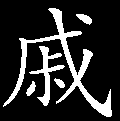
\includegraphics[width=3mm]{../Images/00005}总评:赵姨痛儿,弄得羞愧满面;柳家惜女,几至鞭楚随身。可知养子种孙自有大体,莫学那溺爱禽犊。柳家婆煮糕烹茶,何等殷勤,未得些儿便宜;秦家婆偷仓盗库,百般赔垫,反伤无数钱财。可知君子安贫,达人知命,原有乐处。}

%{\href{../Text/part0065_split_000.html\#navto_1_a}{①}``情赃''、``情权'',除戚本``情权''作``徇私''外,诸本均同。程甲本始改为``瞒赃''、``行权''。}
